\section{In-silico results}\label{sec:results}

\subsection{Estimation under sparse labels}\label{sec:table1}

Eight independent truth realizations were simulated for 90 days each.
Sensors were trained on the first 60 days of labels and evaluated on
the final 30, following the per-plant temporal protocol.
Table~\ref{tab:ablation} summarizes the ablation triple.
% SOURCE: results/table1_summary.csv (commit-regenerable)
\begin{table}[t]\centering
\caption{Estimation ablation on unseen test windows: RMSE in
$\log(1{+}\cdot)$ rate space (mean $\pm$ sd over 8 plants) and the
fraction of estimates within a factor of two of the hidden truth.
Source: \texttt{results/table1\_summary.csv}.}
\label{tab:ablation}
\begin{tabular}{lccc}
\toprule
Arm & RMSE$_{\log 1p}$ & vs.\ physics & within $\times 2$ \\
\midrule
Physics core & $0.196 \pm 0.110$ & --- & 41\% \\
Pure ML & $0.227 \pm 0.086$ & $+16\%$ & 37\% \\
Hybrid (this work) & $\mathbf{0.117 \pm 0.045}$ & $\mathbf{-40\%}$ & \textbf{63\%} \\
\bottomrule
\end{tabular}
\end{table}
The hybrid reduces error by 40\% against its own physics prior and by
48\% against the pure-data baseline. The label-scarcity sweep in
Fig.~\ref{fig:scarcity} sharpens the point. With ten days of labels the
hybrid (0.161) already outperforms the physics core given any amount of
data (0.196), while the pure-data arm needs the full sixty days to
approach what the hybrid achieves in ten. The transfer experiment then
bounds the claim honestly: a residual carried to a foreign plant along
with its donor credibility does active harm (0.317 against the physics
prior's 0.155). This is exactly why $\lambda$ must be earned from the
target plant's own labels. At zero labels $\lambda = 0$ and the hybrid
simply is its prior. The credibility mechanism is the deployment safety
interlock, not decoration.

\begin{figure}[t]\centering
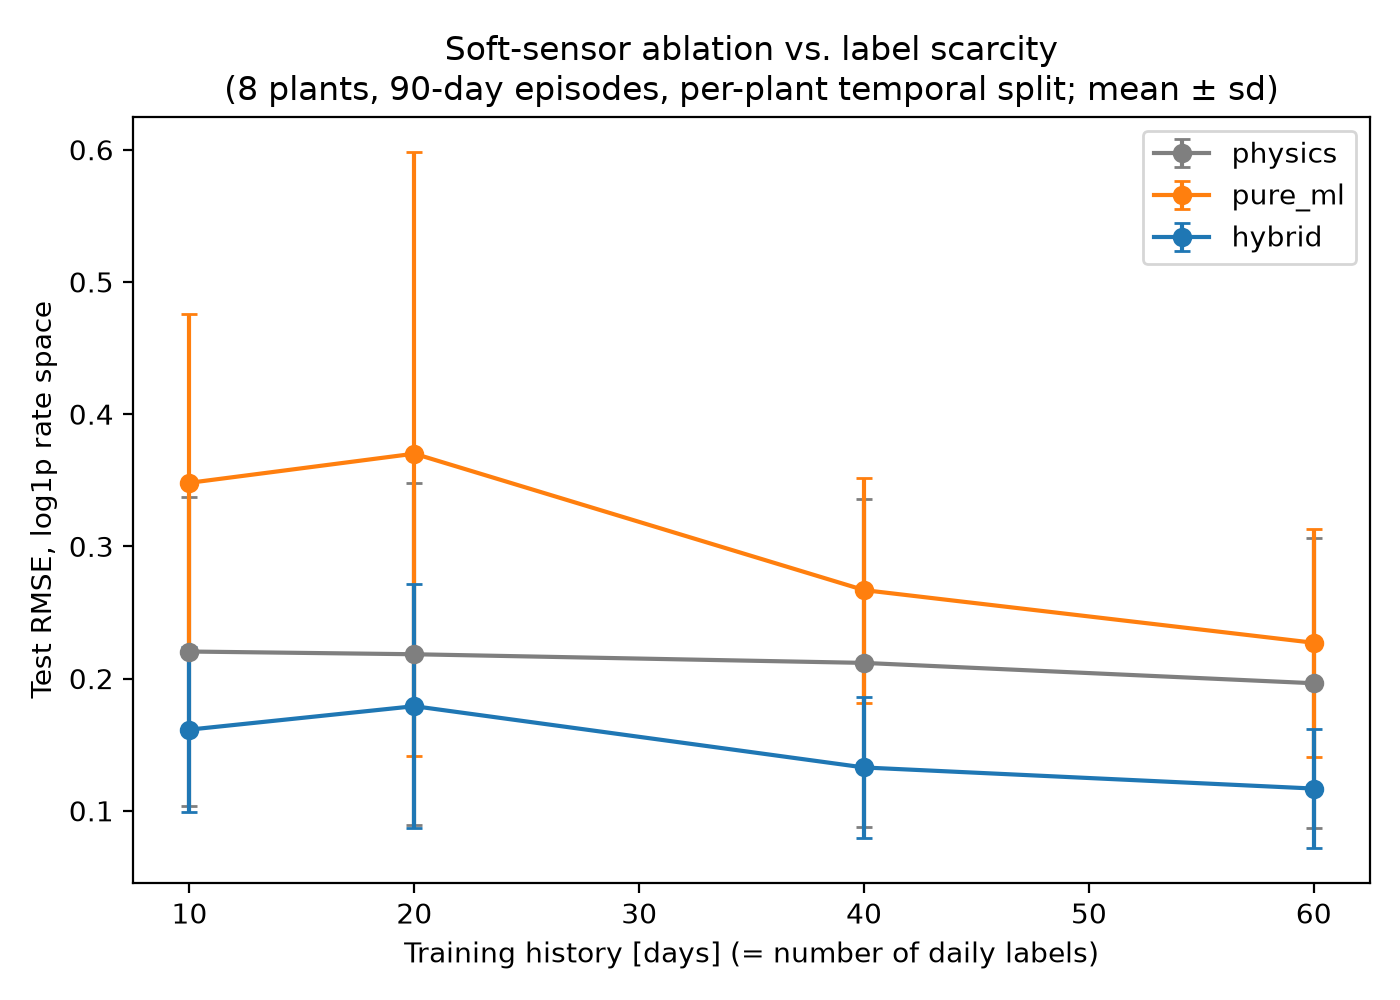
\includegraphics[width=.7\linewidth]{fig_scarcity_sweep.png}
\caption{Test RMSE versus training-history length, equal to the number
of daily labels; mean $\pm$ sd over 8 plants. Source:
\texttt{results/scarcity\_sweep.csv}.}\label{fig:scarcity}
\end{figure}

\subsection{Closed loop under benign mismatch}\label{sec:table2}

Table~\ref{tab:control} reports the four-arm closed-loop benchmark on
six plants over 45 days each: a fixed empirical-practice baseline at
150~$^{\circ}$C and 1~ppm continuous dosing, the pattern of documented
field programs~\citep{baltazar2014grc}; the vertex-robust RTO without
feedback; the scalar-MA loop; and the proposed hybrid-in-the-loop
controller.
% SOURCE: results/table2_summary.csv
\begin{table}[t]\centering
\caption{Closed-loop benchmark in the benign regime (random per-plant
mismatch; 6 plants $\times$ 45 d). Violation days count days whose
realized trailing-24-h mean rate exceeded $r_{\max}$.
Source: \texttt{results/table2\_summary.csv}.}
\label{tab:control}
\begin{tabular}{lcccc}
\toprule
Arm & Gross MW & Uplift & Viol.\ days (max) & Inhib.\ PHP/MWh \\
\midrule
Baseline (fixed) & 5.03 & --- & 0.00 (0) & 85.9 \\
RTO, no feedback & 7.12 & $+41.7\%$ & 0.17 (1) & 51.6 \\
RTO + scalar MA & 9.26 & $+84.1\%$ & 5.33 (12) & 41.2 \\
RTO + hybrid, $\kappa{=}1$ & 6.71 & $+33.4\%$ & \textbf{0.00 (0)} & 53.5 \\
\bottomrule
\end{tabular}
\end{table}
Three observations follow. Even the robust open-loop RTO leaks: one
plant, one violation day, because an envelope over brine chemistry does
not certify against kinetic draws. The scalar-MA loop harvests
spectacularly and unsafely, posting $+84\%$ uplift at an average of
5.33 violation days per plant and twelve on the worst plant, in the
benign regime. The hybrid controller is violation-free on all six
plants; its $+33\%$ uplift sits 8 percentage points below the
no-feedback RTO, and that gap is the premium of the $\kappa\sigma$
back-off. It is the price of insurance, quantified.

\subsection{Adverse-kinetics stress}\label{sec:stress}

The stress magnitude is a measurement, not a choice. The out-of-sample
validation of Section~\ref{sec:validation} finds a sixfold median gap
between the fitted core and independent modern kinetics, so the stress
sets the plant's true rate six times above the model as a deterministic
single-factor perturbation with all random draws zeroed.
Table~\ref{tab:stress} reports the pre-registered outcome.
% SOURCE: results/table2b_summary.csv
\begin{table}[t]\centering
\caption{Adverse stress at the measured sixfold kinetic gap
(single-factor; 6 plants $\times$ 45 d). ``Post-w.'' counts violation
days after the 8-day warm-up. Source:
\texttt{results/table2b\_summary.csv}.}
\label{tab:stress}
\begin{tabular}{lcccc}
\toprule
Arm & Uplift & Viol.\ days & Post-w. & Net kPHP/h \\
\midrule
Baseline (fixed) & --- & 0.00 & 0.00 & 27.2 \\
RTO, no feedback & $+41.7\%$ & 20.67 & 17.17 & 38.8 \\
RTO + scalar MA & $+37.0\%$ & 16.50 & 14.17 & 37.5 \\
RTO + hybrid, $\kappa{=}0$ & $+21.0\%$ & 4.33 & 2.17 & 33.1 \\
RTO + hybrid, $\kappa{=}1$ & $+6.2\%$ & \textbf{2.67} & \textbf{0.50} & 29.1 \\
\bottomrule
\end{tabular}
\end{table}
The no-feedback RTO violates chronically, on 17.2 of 37 post-warm-up
days: its vertex envelope covers brine uncertainty, not kinetic
mismatch. The scalar-MA loop barely improves on open loop (14.2), and
the mechanism is now precise. An additive bias correction learned at
one operating point cannot stabilize a multiplicative error on a
quartic constraint; the absolute error it measures is small when the
plant runs hot and explodes when the optimizer moves cold, so the loop
hunts and violates in a limit cycle. The hybrid constraint, being
state-dependent, extrapolates structurally. Even without margin
($\kappa{=}0$) it cuts post-warm-up violations eightfold, to 2.17 days.
Our pre-registered target for that arm was zero, and it was not met; we
report the miss. The uncertainty back-off ($\kappa{=}1$) closes the
remainder to 0.50 days at a further harvest cost, which we read as an
honest frontier point: under a sixfold kinetic error there is little
harvest that is safe to take. We also observe the optimizer
substituting the dose lever for the temperature lever once the latter
becomes risk-expensive, with inhibitor intensity falling to
38--45~PHP/MWh on several stressed plants. Across both regimes the
conclusion is a two-by-two. Open-loop robustness is safe but blind,
scalar adaptation is reactive but unsafe, and only the
credibility-weighted hybrid with back-off remains essentially
violation-free in both.

\subsection{Global sensitivity and economic ranges}\label{sec:sobol}

A Sobol study ($N = 512$, seeded, 9{,}216 evaluations) spans the
declared uncertainty set: a kinetic band equal to the measured sixfold
gap, a solubility band equal to the measured endpoint spread
$[0.90, 1.37]$, and declared scenario bands for flash, dose--response,
$r_{\max}$ and economics (Fig.~\ref{fig:sobol}). Kinetic model-family
uncertainty dominates the economics, with total-order indices of 0.41,
0.57 and 0.33 on gross power, optimal temperature and net objective.
The quantity the sensing layer reduces is the quantity that moves the
money. The optimal dose is governed instead by dose--response knowledge
($S_T = 0.67$), which identifies inhibitor characterization as the
second identification target. Feasibility holds at 100\% across the
set, so the declared uncertainty never strands the optimizer, and the
gross-power optimum spans 6.0/11.7/17.6~MW
($q_{05}/q_{50}/q_{95}$). Finally, re-valuing the committed closed-loop
trajectories over the economics envelope attaches ranges to every peso
figure. The enabling assumption is verified rather than assumed: the
optimum moves zero grid steps across all eight envelope corners, with
inhibitor cost below 15\% of revenue everywhere, so uplift percentages
and violation counts are untouched. The safety conclusions of
Tables~\ref{tab:control} and~\ref{tab:stress} do not depend on economic
assumptions.

\begin{figure}[t]\centering
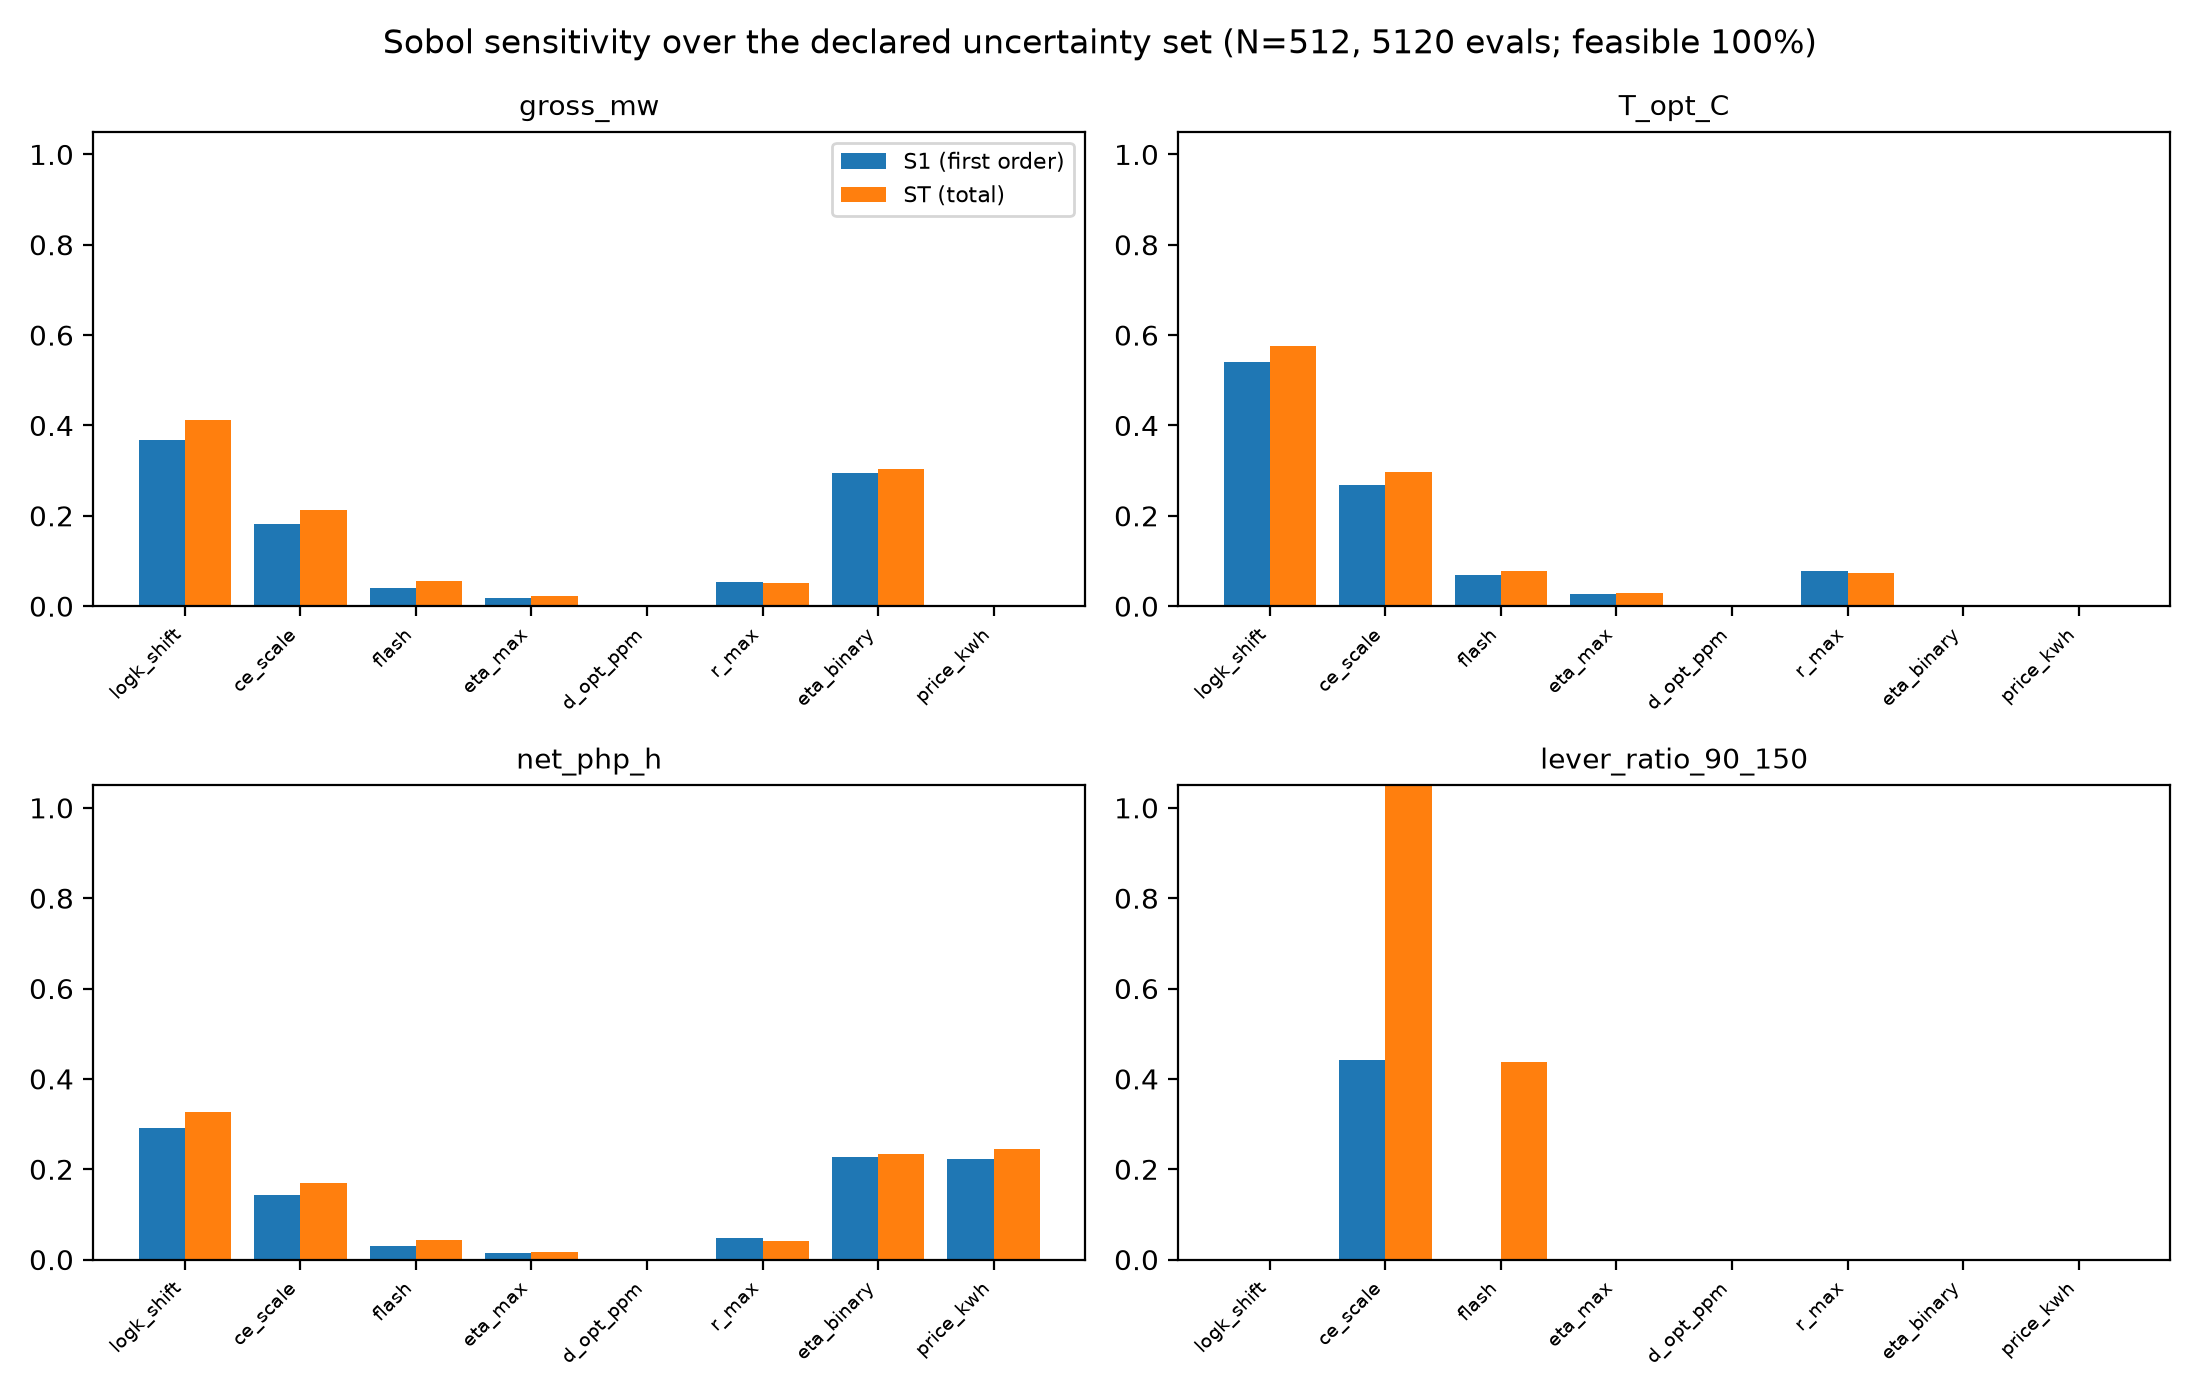
\includegraphics[width=.95\linewidth]{fig_sensitivity_sobol.png}
\caption{First- and total-order Sobol indices over the declared
uncertainty set. Source: \texttt{results/sensitivity\_sobol.csv}.}
\label{fig:sobol}
\end{figure}
